% ch26-cute-ffpa.tex — 撰写任务见 RFC.md F7
\chapter{CuTe 应用（三）：FFPA Split-D 的类型代数}\label{ch:26}

\section{本章导读}

第~\ref{ch:19}~章把 Split-D 当作\emph{算法}讲透了：为什么大 head\_dim 会触及
smem 容量上限、$S$ 如何沿 $D$ 切成 chunk、$O$ 如何拆成分量并在收尾合并、chunk 数与
流水级数的相位关系如何推导。本章换一个视角：把同一份代码（\texttt{ffpa\_\allowbreak{}attn.\allowbreak{}cuh}
的 CuTe 版）当作\emph{类型系统}来读，回答一个第~\ref{ch:19}~章刻意没有展开的问题：

\begin{quote}
  Split-D 的每一个结构决策（双 TiledMma、chunk 循环、独立 $O$ 累加器），
  在 CuTe 里究竟长什么\emph{类型}？哪些事实可以在 host 端离线断言，
  而不必等到 device 上跑出错误结果？
\end{quote}

这个视角有直接的工程收益。第~\ref{ch:25}~章已经演示过一次：手写 attention 里靠注释和
规则维持的 lane 映射、tile 计数、转置视图，在 CuTe 版里变成了
\texttt{print\allowbreak{}(layout)} 可以打印、\texttt{static\_\allowbreak{}assert} 可以断言、host 端
测试可以离线核对的\emph{类型事实}。FFPA 把这件事推得更远一步：Split-D 引入的
chunk 循环让归约维度被切开这件事也必须落在类型上：

\begin{itemize}[itemsep=2pt,topsep=2pt]
  \item QK 与 PV 用\emph{两个不同形状}的 TiledMma，却共享同一批 128 个线程；
        两个 fragment 为什么能免 smem 交接？
  \item $S$ 的归约维（$D$）被切成 $C$ 个 chunk，但 $S$ 的 fragment 形状
        \emph{一次都没有变}，chunk 循环到底切开了什么？
  \item 每个 chunk 一份 $O$ 累加器，$C\times 32$ 个 f32 逻辑累加值是怎么被
        类型推导出来的？
\end{itemize}

本章的叙述顺序与第~\ref{ch:25}~章一致：先给类型代数（26.3 节，所有公式都能
在 host 端用 CuTe 原语验证），再逐相位读 kernel（26.4 节），最后是常见坑、
面试速查与最小测试。全章沿一条数据流展开：Q/K 的 chunk 从 smem
切片进来、在 $S$ 的 32 个寄存器里跨 chunk 累加、经 rowcol 视图做 online
softmax 就地写回 $S$，再由 \texttt{convert\_type} 产生 f16 fragment、用 Aregs
重解释成 PV 的 A 操作数。每一步都只用
\emph{类型}回答数据在哪、什么形状、谁持有。两处布局变换（rowcol 与
Aregs）的通用讲法在第~\ref{ch:25}~章 25.3.4 节已经展开，本章只补 Split-D
语境下的增量。涉及算法推导（chunk 分解的数学、online softmax 的不变量、
相位计数）的地方，直接引用第~\ref{ch:19}~章，不重复。

前置：第~\ref{ch:19}~章（Split-D 算法）、第~\ref{ch:20}--\ref{ch:22}~章
（布局代数、TiledCopy、TiledMMA）、第~\ref{ch:25}~章（attention 的 CuTe 化，
包括共享层 \texttt{convert\_\allowbreak{}layout\_\allowbreak{}acc\_\allowbreak{}rowcol} 与 \texttt{convert\_\allowbreak{}layout\_\allowbreak{}acc\_\allowbreak{}Aregs}
的来历）。

\section{问题与动机}

Split-D 的动机在源头注释里写得很直白（\texttt{ffpa\_\allowbreak{}attn.\allowbreak{}cuh} L7--8）：
\textbf{支持 head\_dim $>128$ 的 large head-dim attention，通过 64-wide Split-D
chunks 处理}。第~\ref{ch:19}~章量化了为什么必须分：smem 容量、以及
$\mathrm{softmax}$ 的结构性位置。本节只关心分完之后抽象层多出的四个问题。

先从第~\ref{ch:25}~章的结论出发。FA2 的三个 CuTe 实现里，attention 的
$D$ 维（head\_dim）是\emph{一个整体}：Q/K/V 的 smem tile 直接是
$[B_r, D]$、$[B_c, D]$，TiledMma 的 $K$ 向一次覆盖 16 列，循环在 $N$（KV tile）
方向滚动。FFPA 把这两件事都改了：

\begin{enumerate}[itemsep=3pt,topsep=3pt]
  \item K 向（$D$）被切成 chunk，循环滚动。$D=512$ 时
        $C = 512/64 = 8$ 个 chunk；QK 的累加变成一个\emph{跨 chunk 的求和}，
        每个 chunk 内部仍是一条标准的 $k16$ MMA 链。
  \item QK 与 PV 的 TiledMma 形状不同。QK 要一次覆盖 $S[64,64]$
        （省掉 N-tile 循环），PV 每次只覆盖 $O$ 的 16 列，
        以缩小单次调用的 C fragment 与临时量；跨 chunk 的 $O$ 总量仍由
        $D$ 与线程数决定。两者共享同一批线程，$S$（QK 的 C fragment）必须
        变成 $P$（PV 的 A 操作数）。
  \item $O$ 的累加器按 chunk 分裂。$D=512$、$C=8$ 时，每个线程
        持有 $8\times32$ 个 f32 的 $O$ 分量。
  \item 生产者也要跟着分 chunk。TMA box 或 cp.async 的搬运单元
        从整块 $[64,D]$ 变成 $C$ 个 $[64,64]$。
\end{enumerate}

四个问题的共同点：它们\emph{都不是数值问题}（数值精度与归约顺序都已确
定），而是\textbf{类型与布局问题}：tile 怎么切、fragment 怎么换解释、寄存器
怎么编号、循环与 stage 怎么对应。把这四个问题逐个翻译成 CuTe 的类型与布局，
就是用 CuTe 抽象表达 Split-D 的全部内容。

本章引用的源码位置汇总在表~\ref{tab:26-code}。

\begin{table}[htbp]
\centering
\caption{本章引用的 \texttt{ffpa\_\allowbreak{}attn.\allowbreak{}cuh} 位置（CuTe 版，cp.async 路径
\texttt{ffpa\_\allowbreak{}split\_\allowbreak{}d\_\allowbreak{}cute}，L79--376）。TMA+WS 版在同构位置复用同一批
helper，差异归第~\ref{ch:19}~章。}
\label{tab:26-code}
\begin{tabular}{p{4.2cm}p{3.4cm}p{6.0cm}}
\toprule
源码位置 & 内容 & 本章视角 \\
\midrule
L42--61 & traits：smem 布局与双 TiledMma & 类型推导链（26.3.1） \\
L79--97 & kernel 签名与 chunk 常量 & 128 线程 / \texttt{kDChunks}（26.4.1） \\
L118--128 & G2S \texttt{TiledCopy} & TV 布局与 MMA 对齐（26.4.2） \\
L136--141 & V 的 fragment 布局预计算 & 转置视图与 nonswizzle（26.4.3） \\
L152--176 & fragment 尺寸与寄存器占用 & 可断言的常量（26.3.2） \\
L217--271 & Phase 1：QK 的 chunk 流水 & 归约维的循环表达（26.4.5） \\
L273--303 & Phase 2：softmax 与 $P$ 的生成 & rowcol 与 Aregs（26.3.3） \\
L307--353 & Phase 3：PV 的 chunk 循环 & 双 TiledMma 的交接（26.4.6） \\
L355--374 & Phase 4：归一化与写回 & 收尾的布局复用（26.4.7） \\
\bottomrule
\end{tabular}
\end{table}

\section{数学原理：类型与布局代数}

\subsection{两个 TiledMma 的推导链}

第~\ref{ch:22}~章给出了 TiledMMA 的三元组
$(\mathrm{Atom},\ \mathrm{AtomLayout},\ \mathrm{Tile})$，以及每线程补足的
atom 重复数（源码注释称之为 \texttt{EURepeat}）：

\begin{equation}
  \mathrm{EURepeat} \;=\; \frac{\mathrm{Tile}}
  {\mathrm{AtomShape}\otimes \mathrm{AtomLayout}} ,
  \qquad
  \mathrm{AtomShape} = (16,8,16),\quad \mathrm{AtomLayout} = (4,1,1).
  \label{eq:26-eurepeat}
\end{equation}

代入两个 Tile（\texttt{ffpa\_\allowbreak{}attn.\allowbreak{}cuh} L52--58）：

\begin{align}
  \text{QK:}\quad & (64,64,16) \oslash \bigl((16,8,16)\otimes(4,1,1)\bigr)
    = (64,64,16)\oslash(64,8,16) = \langle 1,8,1\rangle ,
  \label{eq:26-qk}\\[2pt]
  \text{PV:}\quad & (64,16,16) \oslash (64,8,16) = \langle 1,2,1\rangle .
  \label{eq:26-pv}
\end{align}

读法：$M$ 向的 4 个 atom 位置被 4 个 warp 分完（$\mathrm{AtomLayout}$ 的
$M$ 分量 $=4$，每 warp 负责 16 行，故 $M$ 向的重复数为 1）；$N$ 向没有
atom-layout 的分工（$N$ 分量 $=1$），所以 $N$ 向的重复数就是
$\mathrm{Tile}_N/8$：QK 是 8，PV 是 2。

\begin{quote}
  $\mathrm{EURepeat}_N$ 就是每个线程每个 k-step 发射的
  \texttt{mma.sync} 条数。\allowbreak{}QK 的 8 条一次覆盖 $S$ 的整个 64 列
  （$8\times n8$），于是 N-tile 循环整个消失；PV 的 2 条只覆盖
  $O$ 的 16 列，$O$ 的其余列由外层 V-chunk 循环驱动。
\end{quote}

图~\ref{fig:26-dual-mma} 把这条对比摆成两个 tile 网格：行维同样被
$\mathrm{AtomLayout}=(4,1,1)$ 的 4 个 warp 分完，列维的 atom 数相差 4 倍。

\begin{figure}[H]
\centering
\begin{tikzpicture}[
  blknum/.style={font=\footnotesize\bfseries, inner sep=1pt},
  axl/.style={font=\scriptsize, inner sep=1pt},
]
  % 行轴：4 warp 分 M=64（AtomLayout=(4,1,1) 的 M 分量 = 4，每 warp 16 行）
  \foreach \wr/\mlo/\mhi in {0/0/15, 1/16/31, 2/32/47, 3/48/63} {
    \node[axl,anchor=east,align=right] at (1.02,-\wr*0.86-0.43)
      {w\wr\\{\tiny $m\,\mlo..\mhi$}};
  }
  % 左网格：S = QK 的输出 tile 64x64（4 warp 行块 x 8 个 n8 atom 列块）
  \foreach \wr in {0,...,3} {
    \foreach \aa in {0,...,7} {
      \pgfmathtruncatemacro{\gra}{12+8*\aa}
      \pgfmathtruncatemacro{\mn}{\aa+1}
      \fill[tkBlue!\gra] (1.1+\aa*1.05,-\wr*0.86) rectangle (1.1+\aa*1.05+1.05,-\wr*0.86-0.86);
      \node[blknum] at (1.1+\aa*1.05+0.525,-\wr*0.86-0.43) {\mn};
    }
  }
  \draw[thick, tkBlue] (1.1,0) rectangle (9.5,-3.44);
  \foreach \wr in {1,2,3} {
    \draw[very thick] (1.1,-\wr*0.86) -- (9.5,-\wr*0.86);
  }
  \foreach \aa in {1,...,7} {
    \draw[thin] (1.1+\aa*1.05,0) -- (1.1+\aa*1.05,-3.44);
  }
  % 右网格：O 的一个 chunk 分量 64x16（4 warp 行块 x 2 个 n8 atom 列块）
  \foreach \wr in {0,...,3} {
    \foreach \aa in {0,...,1} {
      \pgfmathtruncatemacro{\gra}{18+30*\aa}
      \pgfmathtruncatemacro{\mn}{\aa+1}
      \fill[tkGreen!\gra] (11.0+\aa*0.95,-\wr*0.86) rectangle (11.0+\aa*0.95+0.95,-\wr*0.86-0.86);
      \node[blknum] at (11.0+\aa*0.95+0.475,-\wr*0.86-0.43) {\mn};
    }
  }
  \draw[thick, tkGreen] (11.0,0) rectangle (12.9,-3.44);
  \foreach \wr in {1,2,3} {
    \draw[very thick] (11.0,-\wr*0.86) -- (12.9,-\wr*0.86);
  }
  \draw[thin] (11.95,0) -- (11.95,-3.44);
  % 顶部标题与 atom 刻度
  \node[font=\scriptsize\bfseries,align=center,text=tkBlue] at (5.3,0.85)
    {QK TiledMma：Tile $=(64,64,16)$\\$\mathrm{EURepeat}=\langle 1,8,1\rangle$};
  \node[font=\scriptsize\bfseries,align=center,text=tkGreen!70!black] at (11.95,0.85)
    {PV TiledMma：Tile $=(64,16,16)$\\$\mathrm{EURepeat}=\langle 1,2,1\rangle$};
  \node[axl,anchor=south,text=tkBlue] at (5.3,0.22) {$S$（每块 = 一个 $n8$ atom，格内数字 = 该 warp 本 k-step 发射的第几条 \texttt{mma.sync}）};
  \node[axl,anchor=south,text=tkGreen!70!black] at (11.95,0.22) {$O$ 的 chunk $c$ 分量};
  \foreach \aa in {0,...,7} {
    \node[axl,anchor=north] at (1.1+\aa*1.05+0.525,-3.52) {\aa};
  }
  \foreach \aa in {0,...,1} {
    \node[axl,anchor=north] at (11.0+\aa*0.95+0.475,-3.52) {\aa};
  }
  \node[axl,anchor=north] at (5.3,-3.95) {atom 列序（$N$ 向，每块 8 列：QK 共 $8{\times}8{=}64$ 列）};
  \node[axl,anchor=north] at (11.95,-3.95) {共 16 列};
  % 交接箭头
  \draw[-{Stealth},thick,tkPurple] (9.72,-1.72) -- (10.78,-1.72);
  \node[font=\scriptsize,anchor=south,text=tkPurple] at (10.25,-1.66) {$P$};
  \node[font=\tiny,align=center,anchor=north,text=tkPurple] at (10.25,-1.78) {softmax\\Aregs 交接};
  % 底部两行注记
  \node[axl,anchor=north west,align=left,text width=11.6cm] at (1.1,-4.35)
    {两个 TiledMma 的 frag 相同：$\mathrm{frag}_S=\mathrm{frag}_O=((2,2),1,8)=32$ 值/线程
     （式~\eqref{eq:26-frag32}，第三 mode 的 8 来历不同）；行维同被 4 warp 分完，};
  \node[axl,anchor=north west,align=left,text width=11.6cm] at (1.1,-5.25)
    {差别全在 $N$ 向：\textcolor{tkBlue}{QK} 的 $\mathrm{EURepeat}_N{=}8$ ——8 条 \texttt{mma.sync} 一次覆盖 $S$ 整个 64 列，\textbf{N-tile 循环}消失；
     \textcolor{tkGreen!70!black}{PV} 的 $\mathrm{EURepeat}_N{=}2$ 只覆盖 $O$ 的 16 列，其余列由外层 V-chunk 循环驱动。};
\end{tikzpicture}
\caption{双 TiledMma 的 Tile 分工（式~\eqref{eq:26-qk}--\eqref{eq:26-pv}）。
左：QK 的输出 $S[64,64]$——4 个 warp 各占 16 行（$\mathrm{AtomLayout}$ 的 $M$ 分量 4），
列向 8 个 $n8$ atom 由\textbf{同一线程}在一个 k-step 里连发 8 条 \texttt{mma.sync} 覆盖
（蓝深浅 8 档标识 atom 身份，格内数字为发射序）；右：PV 的输出 $O$ 只有一个
chunk 分量 $[64,16]$（绿 2 档、2 个 atom、2 条 \texttt{mma.sync}）。中间箭头是 26.3.3 节的
交接：$S$ 经 softmax 后由 \texttt{convert\_type} 转成 f16 fragment，
\texttt{Aregs} 再重解释其布局作为 PV 的 A 操作数；全程不经过 smem。}
\label{fig:26-dual-mma}
\end{figure}

对照第~\ref{ch:25}~章 FA2 traits 的 $(8,1,1)\otimes(128,16,16)$：那里是
8 个 warp 分 $M=128$，$N$ 向重复数为 2。同一套公式，两种分工：FA2 把线程
堆在 $M$ 上换取更大的 $B_r$；FFPA 仍是 4 个 warp 分 $M=64$，$N$ 向没有
atom-layout 分工，一次覆盖整行块 $S$ 靠的是同一线程的
$\mathrm{EURepeat}_N=8$，不是把线程堆到 $N$ 上。

\subsection{fragment 的元素计数：两个恒等式}

TiledMma 定下来之后，每个线程持有多少寄存器就定了。这里有两个恒等式，后面
要讲的免 smem 交接就建立在它们上。

\textbf{恒等式一（C fragment 的大小）}：
\texttt{partition\_\allowbreak{}fragment\_\allowbreak{}C} 把\emph{目标输出形状}按 TiledMma 的线程布局
切开，所以

\begin{equation}
  \bigl|\mathrm{frag}_C\bigr| \;=\;
  \frac{\bigl|\text{目标输出形状}\bigr|}{\text{线程数}} .
  \label{eq:26-csize}
\end{equation}

FFPA 的两处调用（L152 与 L218）目标形状都是 $(64,64)$，线程数都是 128，
所以 QK 的 $S$ 与 PV 的 $O$ 都是每线程 32 个 f32。实测：

\begin{equation}
  \mathrm{frag}_S = \bigl((2,2),1,8\bigr) = 32\ \text{值/tid},\qquad
  \mathrm{frag}_O = \bigl((2,2),1,8\bigr) = 32\ \text{值/tid} .
  \label{eq:26-frag32}
\end{equation}

注意 $\mathrm{frag}$ 的第三 mode 是 8：那是 QK 的 $\mathrm{EURepeat}_N$
在 $S$ 上的投影。$O$ 的第三 mode 数字恰好也是 8，但它来自目标输出
$64$ 列按每个 $n8$ atom 分出的 $8$ 个列组（$64/8{=}8$），
不是 $\mathrm{EURepeat}_N$ 的 $8$。两个 32 的来历不同、大小相同，
这是 $S\to P$ 与 $P\to O$ 两条交接链路能成立的前提。

恒等式二（rowcol 视图的行列数）：online softmax 要在
行上做 max/sum，所以第~\ref{ch:25}~章的工具函数
\texttt{convert\_\allowbreak{}layout\_\allowbreak{}acc\_\allowbreak{}rowcol} 把 $C$ fragment 从
$(\mathrm{MMA}=4,\ \mathrm{MMA\_M},\ \mathrm{MMA\_N})$ 重排成
$\bigl((2,\mathrm{MMA\_M}), (2,\mathrm{MMA\_N})\bigr)$。FFPA 用它推两个
常量（L158--162）：

\begin{equation}
  \mathrm{nrow} = 2\cdot\mathrm{MMA\_M} = 2, \qquad
  \mathrm{ncol} = 2\cdot\mathrm{MMA\_N} = 16 .
  \label{eq:26-rowcol}
\end{equation}

$\mathrm{nrow}=2$ 的含义：\emph{每个线程只拥有 2 行}，行内 16 列。
$n16$ 的 $C$ fragment 里，一个线程的 4 个值的一半（行偏移 $+8$ 的那对）
属于另一行；4 个线程（lane 的 $\text{id}/4$ 相同、$\text{id}\bmod 4$ 不同）
拼成完整的一行，源码里行归约只用 \texttt{\_\allowbreak{}\_\allowbreak{}shfl\_\allowbreak{}xor\_\allowbreak{}sync} 掩码 1 与 2
（后者把 4 个 lane 的两两组合并），原因就在这里。第~\ref{ch:25}~章在手写版
同步链里数过的谁和谁在同一行，在 FFPA 里被压缩成两个常量。

\subsection{$S \to P$：免 smem 的布局重解释}

$S$（QK 的 C fragment，f32）要变成 PV 的 A 操作数 $P$（f16）。两步操作
（L301--303）：

\begin{enumerate}[itemsep=2pt,topsep=2pt]
  \item \texttt{convert\_\allowbreak{}type\allowbreak{}<Element>\allowbreak{}(t\allowbreak{}Cr\allowbreak{}S)}：用
        \texttt{NumericArrayConverter} 做 f32$\to$f16 数值转换，并产生新的
        f16 fragment；它只作用于底层平坦数组，不按当前 layout 的连续段分组。
  \item \texttt{convert\_\allowbreak{}layout\_\allowbreak{}acc\_\allowbreak{}Aregs\allowbreak{}<Tiled\allowbreak{}Mma\allowbreak{}PV>\allowbreak{}(layout)}：把布局
        重解释成 $m16n8k16$ 的 A 操作数布局；这一步不搬动底层数组。
\end{enumerate}

源码先做类型转换、再做 Aregs；但两者不是按 layout 连续段绑定的。转换器只
看到底层平坦数组，Aregs 只重解释索引，所以不能把“反序会按错误连续段分组”
当作顺序理由。Aregs 本身调用的就是第~\ref{ch:25}~章 25.3.4 节精读过的那个
\texttt{convert\_\allowbreak{}layout\_\allowbreak{}acc\_\allowbreak{}Aregs}
（Tri Dao 的 \texttt{logical\_\allowbreak{}divide} 几何法与 @reed 的
inverse$\circ$compose 代数法都在讲同一件事）。放到 Split-D 的语境里，
补三点增量：

\begin{itemize}[itemsep=2pt,topsep=2pt]
  \item \textbf{为什么免 smem 往返}：$S$ 的 32 个寄存器是 Phase 2 最紧张
        的资源，softmax 之后直接转换成 $P$；若改走 $P$ 写回 smem 再
        ldmatrix，每个 kv\_tile 在完整 QK 与 softmax 之后会多出一次
        $64\times64$ 的 half 往返与一次同步。这笔开销按 kv\_tile 数计，
        不随 D-chunk 数 $C$ 成倍增加。
  \item \textbf{为什么模板参数是 \texttt{\allowbreak{}<Tiled\allowbreak{}Mma\allowbreak{}PV>}}：Aregs 重解释要按
        \emph{消费者}的 atom 约定推：PV 的 $k16$ atom 决定 K 向 2 值
        落在哪个寄存器编号上，而不是 QK 的约定。
  \item \textbf{数据流本身}：$S$ 的列（$B_c$ 向）在 $P$ 里变成 K 向，而
        $PV$ 的归约恰好沿这个方向；$P$ 的生产者（softmax）与消费者（PV）
        作用在同一维上，变换只调整哪个寄存器读哪一对列。
\end{itemize}

第二步为什么合法？在 atom 一级看两个 fragment 的\emph{线程-值}映射
（第~\ref{ch:22}~章符号；$m$ 行、$k$ 是 $P$ 的 K 向 $=S$ 的列）：

\begin{align}
  C\ (m16n8):\quad & m = \frac{lane}{4} + 8d_1,\quad
    n = 2\,(lane\bmod 4) + d_0, \qquad v = d_0 + 2d_1, \label{eq:26-cmap}\\
  A\ (m16k16):\quad & m = \frac{lane}{4} + 8d_1,\quad
    k = 2\,(lane\bmod 4) + d_0 + 8d_2, \qquad v = d_0 + 2d_1 + 4d_2 .
  \label{eq:26-amap}
\end{align}

把式~\eqref{eq:26-cmap} 的 $C$ 映射沿值方向拆位：低 2 个值（$v=0,1$，即 $(d_0,d_1)=(0,0),(1,0)$）
是\emph{同一行、相邻两列}（$d_0$ 即列 $+1$）；高 2 个值（$d_1=1$）是
行 $+8$ 的另一对。而式~\eqref{eq:26-amap}
的 $A$ 映射里，$d_0$ 同样是 k 向相邻 2 值。于是 C 的 4 个值与
A 的 4 个值在寄存器里一一对应：A 的 $k$ 向 2 值 $=$ C 的
列向 2 值，A 的行维与 C 的行维本来就一致。第~\ref{ch:25}~章把这条性质
记作\textbf{不是通用性质，换 atom 必须重推}（源码 L2360 附近的注释）；在 FFPA
里它的意义更重：$P$ 的 K 向就是 $S$ 的列向，而那一维正是 PV 的
归约维，重解释的方向恰好对齐 MMA 的约定，所以不需要 shuffle、
不需要过 smem。

图~\ref{fig:26-camap} 把这两条映射放到同一批格子上逐位核对：
同一个 lane 在两图里高亮的位置完全相同，变的只是值编号与分组。

\begin{figure}[H]
\centering
\begin{tikzpicture}[
  cfl/.style={font=\tiny, inner sep=0.2pt},
  axl/.style={font=\scriptsize, inner sep=1pt},
  nt/.style={font=\scriptsize, align=left, inner sep=1.5pt},
]
  % 左：C 视图 m16 x 16（两个 n8 atom 拼成）；高亮 lane 6 的 8 个值
  \foreach \rr in {0,...,15} {
    \foreach \cc in {0,...,15} {
      \pgfmathtruncatemacro{\hit}{(\rr==1 || \rr==9) && (\cc==4 || \cc==5 || \cc==12 || \cc==13) ? 1 : 0}
      \ifnum\hit=1
        \fill[colorx6!45] (\cc*0.42,-\rr*0.42) rectangle (\cc*0.42+0.41,-\rr*0.42-0.41);
        \draw[thick,colorx6!75!black] (\cc*0.42,-\rr*0.42) rectangle (\cc*0.42+0.41,-\rr*0.42-0.41);
      \else
        \filldraw[fill=gray!22, draw=gray!55, thin] (\cc*0.42,-\rr*0.42) rectangle (\cc*0.42+0.41,-\rr*0.42-0.41);
      \fi
    }
  }
  \foreach \rr/\cc/\vv in {1/4/0, 1/5/1, 9/4/2, 9/5/3, 1/12/0, 1/13/1, 9/12/2, 9/13/3} {
    \node[cfl,font=\tiny\bfseries] at (\cc*0.42+0.205,-\rr*0.42-0.205) {\vv};
  }
  \draw[thick] (0,0) rectangle (6.72,-6.72);
  \draw[very thick] (3.36,0) -- (3.36,-6.72);
  \foreach \rx in {0,4,8,12,15} {
    \pgfmathsetmacro{\ry}{-\rx*0.42-0.21}
    \node[axl,anchor=east] at (-0.1,\ry) {\rx};
  }
  \node[axl,anchor=south,rotate=90] at (-0.66,-3.36) {行 $m$};
  \node[axl,anchor=north] at (1.68,-6.85) {$n8$ atom 0};
  \node[axl,anchor=north] at (5.04,-6.85) {$n8$ atom 1};
  \node[axl,anchor=north] at (3.36,-7.35) {C 视图：列 $n$（$S$ 的 $B_c$ 向）};
  % 中间：同一批寄存器
  \node[axl,rotate=90] at (7.66,-3.36) {同一批 f16 寄存器，换 A 的约定读（布局重解释）};
  % 右：A 视图 m16 x 16（一个 k16 atom）
  \foreach \rr in {0,...,15} {
    \foreach \cc in {0,...,15} {
      \pgfmathtruncatemacro{\hit}{(\rr==1 || \rr==9) && (\cc==4 || \cc==5 || \cc==12 || \cc==13) ? 1 : 0}
      \ifnum\hit=1
        \fill[colorx6!45] (\cc*0.42+8.6,-\rr*0.42) rectangle (\cc*0.42+9.01,-\rr*0.42-0.41);
        \draw[thick,colorx6!75!black] (\cc*0.42+8.6,-\rr*0.42) rectangle (\cc*0.42+9.01,-\rr*0.42-0.41);
      \else
        \filldraw[fill=gray!22, draw=gray!55, thin] (\cc*0.42+8.6,-\rr*0.42) rectangle (\cc*0.42+9.01,-\rr*0.42-0.41);
      \fi
    }
  }
  \foreach \rr/\cc/\vv in {1/4/0, 1/5/1, 9/4/2, 9/5/3, 1/12/4, 1/13/5, 9/12/6, 9/13/7} {
    \node[cfl,font=\tiny\bfseries] at (\cc*0.42+8.805,-\rr*0.42-0.205) {\vv};
  }
  \draw[thick] (8.6,0) rectangle (15.32,-6.72);
  \draw[dashed,very thick] (11.96,0) -- (11.96,-6.72);
  \foreach \rx in {0,4,8,12,15} {
    \pgfmathsetmacro{\ry}{-\rx*0.42-0.21}
    \node[axl,anchor=east] at (8.5,\ry) {\rx};
  }
  \node[axl,anchor=south,rotate=90] at (7.94,-3.36) {行 $m$};
  \node[axl,anchor=north] at (10.28,-6.85) {$d_2{=}0$};
  \node[axl,anchor=north] at (13.64,-6.85) {$d_2{=}1$};
  \node[axl,anchor=north] at (11.96,-7.35) {A 视图：K 向 $k$（$PV$ 归约维，一个 $k16$ atom）};
  % 底部：两条映射式
  \node[nt,anchor=north west,text width=15.6cm] at (0,-7.65)
    {C（$m16n8$）：$m=\frac{lane}{4}+8d_1$、$n=2\,(lane\bmod4)+d_0$、$v=d_0+2d_1$；
     A（$m16k16$）：$m$ 同式、$k=2\,(lane\bmod4)+d_0+8d_2$、$v=d_0+2d_1+4d_2$
     （式~\eqref{eq:26-cmap}/\eqref{eq:26-amap}）。示例 lane$=6$：两图高亮的 8 格位置逐格相同
     （$m\in\{1,9\}$、列 $\{4,5\}\cup\{12,13\}$），C 的值编号在两个 atom 内各自 $0..3$ 循环，
     A 因多出 $d_2$ 而连续成 $0..7$——\textbf{A 的 K 向 2 值 $=$ C 的列向 2 值，行维本来就一致}。};
\end{tikzpicture}
\caption{C 与 A fragment 的线程-值映射逐位对照（式~\eqref{eq:26-cmap}/\eqref{eq:26-amap}）。
左：$S$ 的 C 视图——两个 $n8$ atom 拼成 16 列，格内数字是 lane 6 所持值的编号
$v=d_0+2d_1$（在每个 atom 内循环 $0..3$）；右：$P$ 的 A 视图——同一个 $k16$ atom，
lane 6 持有同样的 8 个格，值编号变成 $v=d_0+2d_1+4d_2$ 连续 $0..7$，其中
$d_2{=}1$ 的 4 格来自 C 的第二个 $n8$ atom（虚线半块）。\textbf{两图高亮位置逐格相同、
数据指针不换}：重解释只把\textbf{列向相邻 2 值}的约定换成\textbf{K 向相邻 2 值}，
行维（$m$）的映射本来就一致。}
\label{fig:26-camap}
\end{figure}

\begin{remark}
  如果 PV 的 atom 换成 SM80 的 $k8$，A 的 K 向只剩 8 列，$S$ 的 16 列要拆成
  两次 PV。但该 atom 的 A 与 C 都使用 \texttt{SM80\_16x8\_Row}，线程--值映射
  相同，所以每次 $k8$ PV 仍可复用布局，不能仅凭少了 $d_2$ 就断言零拷贝失效。
  换成 wgmma 等其他操作数约定时才需另推。第~\ref{ch:19}~章讨论过的
  \textbf{QK 与 PV 能不能共用一份 $P$}，判据是目标 atom 的 A/C 映射是否兼容。
\end{remark}

\subsection{D-chunk 循环的布局语义}

最后一个代数问题是 chunk 循环切开了什么。先给结论：

\begin{quote}
  Split-D 不改变任何 fragment 的形状，它改变的是\emph{循环结构}和
  \emph{归约树}。
\end{quote}

看 $S$ 的归约：$S = QK^{\top}$ 的真形式是 $S_{ij} = \sum_{d=0}^{D-1}Q_{id}K_{jd}$。
数值上它是一条长 $K$ 向链；结构上 FFPA 把它组织成两级：

\begin{equation}
  S_{ij} \;=\; \sum_{c=0}^{C-1}\ \underbrace{\sum_{t=0}^{3}\sum_{s=0}^{15}
  Q_{i,\,64c+16t+s}\,K_{j,\,64c+16t+s}}_{\text{chunk } c\ \text{内部：4 个 } k16\ \text{atom}} ,
  \qquad C = \frac{kHeadDim}{64} .
  \label{eq:26-splitd}
\end{equation}

式~\eqref{eq:26-splitd} 的两级结构在代码里对应两种不同的机制：

\begin{itemize}[itemsep=2pt,topsep=2pt]
  \item \textbf{chunk 内部}：\texttt{gemm\_ss} 的 K 循环（第~\ref{ch:25}~章
        共享层函数），循环上界来自 A fragment 的布局
        $\mathrm{size}<2>(\mathrm{frag}_A)=4$，即\emph{布局决定循环次数}。
  \item \textbf{chunk 之间}：\texttt{tCrS} 在 chunk 循环外声明、循环内\emph{累加}
        （L218 与 L237--270），归约体现为同一个寄存器数组跨迭代存活。
\end{itemize}

第二点的意义：$S$ 的 fragment 从头到尾是 32 个寄存器，chunk 循环每轮往
它们里面\emph{加}一棵 QK 子树，形状不变、只叠循环。$O$ 的处理不同，但不是
把各 $O_c$ 相加：$O$ 的 D 维被切成互不相交的列块，每个 $O_c$ 只对应其中
一块输出列；Phase 4 对每个分量独立归一化，再写回该列块。$S$ 的 chunk 是
\emph{归约维上的部分和}，必须先求和再做完整 softmax；$O$ 的 chunk 是
\emph{输出维上的分块}，各块保留同一行的 softmax 统计量。第~\ref{ch:19}~章
从数值角度论证过这一点，这里从类型角度再确认：$S$ 是一个 fragment 多次
迭代，$O$ 是多个 fragment 各存一份，代码形状（\texttt{tCrS} vs
\texttt{o\_\allowbreak{}acc\_\allowbreak{}storage[v]}）如实反映了这一点。
图~\ref{fig:26-splitd-struct} 把两者画成“归约树”与“输出列块树”的对比：
左边全部 chunk 汇进同一批 32 寄存器，右边每个 chunk 各占一份存储并写到
不同的 D 列块。

\begin{figure}[H]
\centering
\begin{tikzpicture}[
  axl/.style={font=\scriptsize, inner sep=1pt},
  tnb/.style={font=\tiny, inner sep=0.5pt},
]
  % 顶部：D 维横条，8 个 64-wide chunk（灰度 8 档），每 chunk 4 个 k16 子块
  \node[axl,anchor=east,align=right] at (0.92,-0.28) {Q/K 的\\$D$ 维};
  \node[axl,anchor=south] at (7.0,0.06)
    {$D=512\ \to\ C=8$ 个 64-wide chunk，每 chunk 内 4 个 $k16$ atom（式~\eqref{eq:26-splitd}）};
  \foreach \cc in {0,...,7} {
    \pgfmathtruncatemacro{\gra}{12+8*\cc}
    \fill[gray!\gra] (1.0+1.5*\cc,0) rectangle (2.5+1.5*\cc,-0.55);
    \foreach \ss in {1,2,3} {
      \draw[thin] (1.0+1.5*\cc+0.375*\ss,0) -- (1.0+1.5*\cc+0.375*\ss,-0.55);
    }
    \ifnum\gra>46
      \node[tnb,white] at (1.75+1.5*\cc,-0.28) {c\cc};
    \else
      \node[tnb] at (1.75+1.5*\cc,-0.28) {c\cc};
    \fi
  }
  \draw[thick] (1.0,0) rectangle (13.0,-0.55);
  % Phase 标签
  \node[axl,anchor=west] at (1.0,-0.95) {\textbf{Phase 1（QK）：$S$ 的跨 chunk 累加}};
  \node[axl,anchor=west] at (7.3,-0.95) {\textbf{Phase 3（PV）：$O$ 的分 chunk 存储}};
  % 左 panel：8 棵 qk 子树汇入单个 S fragment
  \foreach \cc in {0,...,7} {
    \pgfmathtruncatemacro{\gra}{12+8*\cc}
    \fill[gray!\gra] (1.0+0.7*\cc,-1.4) rectangle (1.6+0.7*\cc,-1.78);
    \node[tnb] at (1.3+0.7*\cc,-1.59) {$qk_{\cc}$};
    \pgfmathtruncatemacro{\gln}{0.6*\gra}
    \draw[-{Stealth},gray!\gln!black,thick] (1.3+0.7*\cc,-1.78) -- (1.3+0.7*\cc,-2.42);
  }
  \node[axl,anchor=west] at (1.0,-1.12) {\tiny 同一批 32 寄存器反复被加：};
  \draw[very thick,tkBlue,fill=tkFillBlue] (1.0,-2.42) rectangle (6.6,-3.32);
  \node[axl] at (3.8,-2.72) {$\mathtt{tCrS}$：32 f32/线程};
  \node[axl] at (3.8,-3.08) {\tiny 跨迭代存活 $\cdot$ 先求和、再 softmax};
  % 右 panel：8 份独立 fragment，Phase 4 逐块归一化写回
  \foreach \cc in {0,...,7} {
    \pgfmathtruncatemacro{\gra}{12+8*\cc}
    \pgfmathsetmacro{\yy}{-1.4-0.34*\cc}
    \fill[gray!\gra] (7.3,\yy) rectangle (7.62,\yy-0.28);
    \pgfmathtruncatemacro{\gfo}{0.4*\gra}
    \pgfmathtruncatemacro{\gln}{0.6*\gra}
    \foreach \gg in {0,...,7} {
      \draw[thin,fill=gray!\gfo] (7.66+0.3*\gg,\yy) rectangle (7.96+0.3*\gg,\yy-0.28);
    }
    \node[tnb,anchor=west] at (7.99,\yy-0.14) {$O_{\cc}$：32 f32/线程};
    \draw[-{Stealth},gray!\gln!black] (10.6,\yy-0.14) -- (11.25,\yy-0.14);
  }
  \node[axl,anchor=west] at (7.3,-1.12) {\tiny \texttt{o\_acc\_storage[c][32]}，各分量独立 rescale：};
  \draw[thick] (7.3,-1.4) rectangle (10.6,-4.12);
  \node[font=\large] at (11.55,-2.6) {逐块};
  \draw[-{Stealth},thick,tkGreen] (11.85,-2.6) -- (12.35,-2.6);
  \draw[very thick,tkGreen,fill=tkFillGreen] (12.35,-2.95) rectangle (14.15,-2.25);
  \node[axl,align=center] at (13.25,-2.6) {Phase 4\\归一化 + 写回};
  % 底部注记与对比标语
  \node[axl,anchor=north west] at (1.0,-3.45)
    {\tiny softmax 必须在\textbf{完整}的 $S$ 上做（第~\ref{ch:19}~章的数值论证）};
  \node[axl,anchor=north west] at (1.0,-3.85)
    {\tiny $S$ 的归约 = 加法进同一批寄存器；$O$ = 输出 D 列块各自归一化写回};
  \node[axl,anchor=north west,align=left,text width=6.1cm] at (7.3,-4.4)
    {\tiny $D{=}512$ 时 $8\times32=256$ 个 f32 逻辑值，已超过每线程 255 个寄存器的上限（见 26.5 节）};
  \node[font=\scriptsize\bfseries,anchor=west] at (1.0,-5.3)
    {对比：$S$ 先沿归约维求和再 softmax $\;\Vert\;$ $O$ 分 D 列块独立写回};
\end{tikzpicture}
\caption{Split-D 改变的是循环结构与归约树，不是 fragment 形状（26.3.4 节）。
顶条：$D=512$ 切成 $C=8$ 个 64-wide chunk（灰度 8 档贯穿全图），每 chunk 内
4 个 $k16$ atom 对应 \texttt{gemm\_ss} 的 K 循环。左：8 棵 QK 子树全部加进
\textbf{同一个} \texttt{tCrS} fragment——\textbf{一个 fragment 多次迭代}，softmax 必须等
求和完成；右：每个 chunk 的 PV 结果各存一份 \texttt{o\_acc\_storage[c][32]}，
对应输出 D 维上不同的 64 列块。Phase 4 对每块独立归一化并写回自己的列块，
不做 $O=\sum_c O_c$。$S$ 与 $O$ 的 32 值/线程形状完全相同，差别在
$S$ 沿归约维跨迭代累加，$O$ 沿输出维分块保存。}
\label{fig:26-splitd-struct}
\end{figure}

最后是 stage 与 chunk 的正交性。chunk 数 $C$ 由 head\_dim 决定，stage 数
$\mathrm{Sk}/\mathrm{Sv}$ 由 smem 预算决定，两者独立。当前源码选择用
\emph{指针算术}表达 stage 池：

\begin{equation}
  \texttt{q\_base} + \texttt{stage}\times \texttt{k\allowbreak{}QChunk\allowbreak{}Elements},
  \qquad
  \texttt{k\allowbreak{}QChunk\allowbreak{}Elements} = \mathrm{cosize}(\mathrm{SmemLayoutQ}) .
  \label{eq:26-stage}
\end{equation}

这是实现选择，不是 CuTe 布局代数的唯一写法。若要在类型里表达真实 stage
池，可以使用 stride 等于 \texttt{kQChunkElements} 的 stage mode；每个 stage
对应池中一块互不重叠的存储。只有把 stage 做成 stride-0 的伪维时才不同：
那表示所有 stage 落到同一元素，\texttt{cosize} 和 partition 的结果自然
不再对应池大小。FFPA 这里把布局限制为单块 chunk，把池偏移留在指针上，
是为了让每个轮转视图的类型保持最简单。

那么切片与流水在代码里具体长什么样？看 QK 主循环（L237--266）：
gmem 侧的 chunk 由 \texttt{local\_tile} 切出（坐标是 $(q\_tile, d\_chunk)$，
$d$ 从 $0$ 滚到 $\mathrm{Sk}{-}1$）；smem 侧每轮把 \texttt{q\_base} 加上
环状槽位偏移 \texttt{qk\_read} $\times$ \texttt{k\allowbreak{}QChunk\allowbreak{}Elements}，重新
包成一个 \texttt{SmemLayoutQ} 的 tensor。类型是常量、指针是变量：每轮更换的
只是槽位基址，tensor 的布局不变。随后 \texttt{partition\_\allowbreak{}fragment\_\allowbreak{}A} 与
\texttt{s2r\_thr\_q} 的 \texttt{partition\_S} 在这个只描述一块 chunk 的视图
上照常工作（两者的参数都是 \texttt{sQ\_stg}）。

对照第~\ref{ch:25}~章的三级搭建，那里 smem 是常驻的几段静态视图，这里换成了
按 stage 轮转的池：对 CuTe 而言两者没有区别，都是带 layout 的 tensor。流水
的推进则是 \texttt{qk\_read}/\texttt{qk\_write} 两个模 $\mathrm{Sk}$ 的计数器加
\texttt{cp\_\allowbreak{}async\_\allowbreak{}wait\allowbreak{}<Sk-2>}，与第~\ref{ch:25}~章实现 1 的组栈策略
同构（细节见 26.4.5 节）。

\section{设计与实现：逐相位读 kernel}

本节按源码的相位顺序读 \texttt{ffpa\_\allowbreak{}split\_\allowbreak{}d\_\allowbreak{}cute}（cp.async 版，128 线程）。
算法流程（V 预取 $\to$ QK chunk 流水 $\to$ softmax $\to$ PV chunk 流水 $\to$
归一化写回）与第~\ref{ch:19}~章一致；本节只标出类型层的要点。

\subsection{traits 与 chunk 常量}

traits 的核心六行（L48--62）如下，它们的类型推导在 26.3.1 节已经算过：

\lstinputlisting[linerange={48-62},firstnumber=auto,
  title={ffpa\_attn.cuh L48-62（MmaAtom、双 TiledMma、两个 copy atom）}]{../ffpa_attn.cuh}

kernel 的入口与 chunk 常量在 L80--97。这一段值得逐行读，因为它把一个
chunk 有多大的全部依赖固定在编译期：

\lstinputlisting[linerange={80-97},firstnumber=auto,
  title={ffpa\_attn.cuh L80-97（128 线程的 launch bounds 与 chunk 常量：kDChunks 由 head\_dim 推出）}]{../ffpa_attn.cuh}

三处类型要点：

\begin{itemize}[itemsep=2pt,topsep=2pt]
  \item \texttt{\_\allowbreak{}\_\allowbreak{}launch\_\allowbreak{}bounds\_\allowbreak{}\_\allowbreak{}(128)} 不是任意的数字，它对应
        TiledMma 的 $\mathrm{AtomLayout}=(4,1,1)$，即 4 个 warp $\times$ 32 lane
        $=128$。改 Tile 的 $M$ 向分工（例如换 $(2,1,1)$）而忘了同步改
        launch bounds，kernel 里所有 \texttt{get\_\allowbreak{}thread\_\allowbreak{}slice(tid)} 的
        语义都会静默错位；
  \item \texttt{kDChunks = kHeadDim / 64}：chunk 宽度 64 \emph{不是}可选参数，
        它就是 SW128 atom 一行（$64$ 个 half $=128$\,B）的宽度。第~\ref{ch:19}~章
        从 swizzle 的角度解释过；类型上，它与 \texttt{Smem\allowbreak{}Layout\allowbreak{}Atom} 是
        同一个常量；
  \item \texttt{k\allowbreak{}QChunk\allowbreak{}Elements =\allowbreak{} cosize\allowbreak{}(Smem\allowbreak{}Layout\allowbreak{}Q\{\})}：池大小从 layout
        \emph{推出}而不是手写。$\mathrm{cosize}$ 对 SW128 布局的实测值是
        $64\times64=4096$（第~\ref{ch:25}~章的 probe 同款），于是三块池的
        基址（L100--103）也是从它算出来的。
\end{itemize}

\paragraph{实践须知}（读这份源码时最容易踩的三个认知坑）：

\begin{itemize}[itemsep=2pt,topsep=2pt]
  \item 头注释的 kernel 清单不全。\texttt{ffpa\_\allowbreak{}attn.\allowbreak{}cuh} L5--6 写
        \textbf{仅定义……\texttt{ffpa\_\allowbreak{}attn\_\allowbreak{}tma\_\allowbreak{}mma\_\allowbreak{}ws\_\allowbreak{}split\_\allowbreak{}d\_\allowbreak{}cute} kernel}，
        但文件里实际有两个 kernel：本节精读的
        \texttt{ffpa\_\allowbreak{}split\_\allowbreak{}d\_\allowbreak{}cute}（cp.async 版，L82）与
        \texttt{ffpa\_\allowbreak{}attn\_\allowbreak{}tma\_\allowbreak{}mma\_\allowbreak{}ws\_\allowbreak{}split\_\allowbreak{}d\_\allowbreak{}cute}（TMA+WS 版，
        L378 起）。读文件时以实际代码为准；
  \item 256 线程只对 TMA+WS 版成立。L14 与 L28 的
        \textbf{128 producer $+$ 128 consumer $=$ 256 total threads}说的是
        TMA+WS 版（与第~\ref{ch:19}~章 TMA+WS 版的划分一致）；
        cp.async 版是
        \textbf{单角色 128 线程}（L73--78 的注释自己写明了）。按 256 去数
        cp.async 版的 warp 会数错。本节的类型推导统一以 L81 的
        \texttt{\_\allowbreak{}\_\allowbreak{}launch\_\allowbreak{}bounds\_\allowbreak{}\_\allowbreak{}(128)} 为准；
  \item EURepeat 是注释词汇、不是接口。与第~\ref{ch:25}~章同族：
        CuTe 公开可断言的是 \texttt{tile\_\allowbreak{}size\_\allowbreak{}mnk} 与 fragment 布局，
        EURepeat$<$1,8,1$>$/$<$1,2,1$>$ 只是 tile 除以
        (atom$\otimes$layout) 那一刻的中间量（26.3.1 节已按这个口径核对）。
\end{itemize}

\subsection{G2S \texttt{TiledCopy}：与 MMA 划分对齐}

搬运的线程划分（L118--128）是本章第一个对齐要点：

\lstinputlisting[linerange={118-128},firstnumber=auto,
  title={ffpa\_attn.cuh L118-128（G2S：128-bit cp.async，线程布局 16$\times$8，值布局 1$\times$8）}]{../ffpa_attn.cuh}

\texttt{make\_\allowbreak{}tiled\_\allowbreak{}copy} 的两个 layout 分别是线程布局 $(16,8):(8,1)$
（128 个线程铺满，行优先）与值布局 $(1,8)$（每线程一次搬 8 个 half
$=128$\,bit，正好是 \texttt{cp.\allowbreak{}async.\allowbreak{}cg.\allowbreak{}shared.\allowbreak{}global} 的 16 字节形态）。
但源码注释（L73--78）里有一句关键的话：

\begin{quote}
  \textit{128 线程：与 TiledMmaQK/PV 的 Layout$\langle4,1,1\rangle$ 一致，
  每个线程在 G2S 和 S2R/MMA 中有唯一分区，消除 256-thread G2S 与
  128-thread MMA 之间的映射不匹配。}
\end{quote}

这是从 384/256 线程的多角色 kernel 演化到 128 线程单角色的直接证据：
线程数一旦与 TiledMma 的 warp 划分一致，G2S 与 MMA 就能使用同一个
\texttt{tid} 坐标系，省掉多角色之间的一层线程映射。但这不是“转换全部
退化”：G2S 的 TiledCopy 线程/值布局与 MMA 的 \texttt{thrfrg} 布局并不相同，
\texttt{partition\_S}/\texttt{partition\_D} 仍要把一种切分映射到另一种切分。
代价是搬运带宽降低一半（128 线程 vs 256），收益是少一层角色映射与同步协调；
第~\ref{ch:19}~章的性能节从吞吐角度讨论过这项开销。

\subsection{V 的转置视图与 fragment 预计算}

PV 要在循环里反复构造 V 的 B 操作数。FFPA 的做法是把 fragment 布局在循环外
算好（L136--141）：

\lstinputlisting[linerange={136-141},firstnumber=auto,
  title={ffpa\_attn.cuh L136-141（V 的 nonswizzle 转置视图与 fragment 布局预计算）}]{../ffpa_attn.cuh}

三行代码，三个层次：

\begin{enumerate}[itemsep=2pt,topsep=2pt]
  \item \texttt{sV0}：smem 上的 \emph{storage} 视图（带 SW128 swizzle 的
        $[64,64]$ 布局）；
  \item \texttt{sVt0\_ns}：取 \texttt{Smem\allowbreak{}Layout\allowbreak{}Vt} 的
        \textbf{nonswizzle portion}，即去掉 swizzle 后的纯行列布局。
        为什么要去掉？因为 \texttt{partition\_\allowbreak{}fragment\_\allowbreak{}B} 推的是
        哪个线程持有 B 的哪个逻辑元素，swizzle 只改变元素的\emph{地址}，
        不改变\emph{归属}；带着 swizzle 推会让 XOR 置换混进逻辑坐标，
        得到的 fragment 布局与真值错位。这是第~\ref{ch:25}~章\textbf{常见坑}
        的同族问题的另一面（那里禁止拿带 swizzle 的视图推寄存器布局）；
  \item \texttt{tCrV\_layout}：把上面那份推导\emph{求值}成一个布局对象，
        循环里只需 \texttt{make\_\allowbreak{}tensor\allowbreak{}(数据指针,\allowbreak{} t\allowbreak{}Cr\allowbreak{}V\_\allowbreak{}layout)} 重新解释。
\end{enumerate}

图~\ref{fig:26-v-dualview} 把这两份视图的分工画在同一张 smem tile 上：
底色是 SW128 的 XOR 置换模式，两条引出箭头分别指向管指针与管归属的两个角色。

\begin{figure}[H]
\centering
\begin{tikzpicture}[
  cfl/.style={font=\tiny, inner sep=0.2pt},
  axl/.style={font=\scriptsize, inner sep=1pt},
  nt/.style={font=\scriptsize, align=left, inner sep=1.5pt},
]
  % smem tile：8 行（一个 swizzle 周期）x 8 个 16B chunk
  \foreach \rr in {0,...,7} {
    \foreach \pp in {0,...,7} {
      \pgfmathtruncatemacro{\lgc}{mod(\pp+\rr,2)+2*mod(div(\pp,2)+div(\rr,2),2)+4*mod(div(\pp,4)+div(\rr,4),2)}
      \pgfmathtruncatemacro{\gra}{8+9*\lgc}
      \fill[gray!\gra] (\pp*0.72,-\rr*0.5) rectangle (\pp*0.72+0.71,-\rr*0.5-0.49);
      \ifnum\lgc>5
        \node[cfl,white] at (\pp*0.72+0.355,-\rr*0.5-0.245) {\lgc};
      \else
        \node[cfl] at (\pp*0.72+0.355,-\rr*0.5-0.245) {\lgc};
      \fi
    }
  }
  \draw[thick] (0,0) rectangle (5.76,-4.0);
  \foreach \rx in {0,7} {
    \node[axl,anchor=east] at (-0.08,-\rx*0.5-0.25) {\rx};
  }
  \node[axl,anchor=south,rotate=90] at (-0.58,-2.0) {行 $r$};
  \foreach \px in {0,7} {
    \node[axl,anchor=south] at (\px*0.72+0.355,0.10) {\px};
  }
  \node[axl,anchor=north] at (2.88,-4.35) {物理 16B chunk 槽位 $p$（一行 $=$ 128\,B $=8$ 槽）};
  % 两条引出箭头
  \draw[-{Stealth},thick,tkBlue] (5.86,-0.9) -- (6.7,-0.9);
  \draw[-{Stealth},thick,tkGreen] (5.86,-2.6) -- (6.7,-2.6);
  \node[draw=tkBlue,rounded corners,fill=tkFillBlue,align=left,font=\scriptsize,
    text width=8.4cm,inner sep=3pt,anchor=west] at (6.8,-1.32)
    {\texttt{tCrVStorage}/\texttt{tCrV}——\textbf{寄存器 fragment}（每线程私有）：
     \texttt{partition\_fragment\_B} 建立线程--值映射，不划分 smem 数据指针。};
  \node[draw=tkGreen,rounded corners,fill=tkFillGreen,align=left,font=\scriptsize,
    text width=8.4cm,inner sep=3pt,anchor=west] at (6.8,-2.95)
    {\texttt{tCrV\_layout}——\textbf{nonswizzle portion}：决定逻辑坐标与 MMA
     约定。S2R 的 smem 地址另由 \texttt{s2r\_thr\_v.partition\_S(sVt\_stg)} 提供。};
  \node[draw,rounded corners,draw=red!70!black,text=red!70!black,align=left,
    font=\scriptsize,text width=8.4cm,inner sep=3pt,anchor=west] at (6.8,-4.15)
    {\textbf{坑一}：拿带 swizzle 的视图推 fragment 布局，XOR 会混进逻辑坐标；
     但 S2R 的 storage 地址仍必须用带 swizzle 的视图计算。};
  % 底部：位公式
  \node[nt,anchor=north west,text width=15.6cm] at (0,-4.85)
    {SW128 的位公式（第~\ref{ch:23}~章）：$\mathrm{phys}=64r+8\cdot\bigl((c/8)\oplus(r\bmod8)\bigr)+(c\bmod8)$
     ——行内 16\,B chunk 号与行号低 3 位异或（8 行一个周期）。格内数字是该槽实际承载的\emph{逻辑}
     chunk（$c/8=p\oplus(r\bmod8)$），灰度跟随逻辑 chunk 身份，于是\textbf{对角线置换}清晰可见；
     实际 tile 是 $64\times64$（$8$ 个周期），此处只画一个周期。};
\end{tikzpicture}
\caption{V 的双视图分工。同一张 SW128 smem tile：
\texttt{tCrVStorage}/\texttt{tCrV} 是每线程私有的寄存器 fragment；
\texttt{tCrV\_layout}（由 nonswizzle portion 推导）决定\textbf{哪个线程持有哪些逻辑元素}。
S2R 的 smem 地址则由 \texttt{s2r\_thr\_v.partition\_S(sVt\_stg)} 用带 swizzle 的
storage 视图计算。SW128 的 XOR 只改地址、不改归属，故 fragment 归属用
nonswizzle 推导；两份视图职责不同，不能互相替代（坑一）。}
\label{fig:26-v-dualview}
\end{figure}

还有一个容易忽略的点：B fragment 的内容对 4 个 M-warp 是\emph{重复}的
（PV 的 K 向 4 个 atom 要被每个 warp 看到），所以
\texttt{partition\_\allowbreak{}fragment\_\allowbreak{}B} 在 128 线程上给出的每线程元素数
（$\ge$ 128）远大于 C 的 32。但每个 warp 的 B fragment 仍是该线程自己的
寄存器副本，重复只会让 CTA 总寄存器成本更高；评估每线程寄存器压力和
逐元素操作成本时必须把它们算进去，不能称为“共享寄存器”。

\subsection{寄存器占用：$32\times C$ 与两个行向量}

源码（L152--176）把每个寄存器都写在类型上：

\lstinputlisting[linerange={152-176},firstnumber=auto,
  title={ffpa\_attn.cuh L152-176（O fragment 的尺寸、rowcol 行列数、行状态与 $C$ 份累加器）}]{../ffpa_attn.cuh}

逐项列出（本节测试在 host 端断言的正是这些数）：

\begin{itemize}[itemsep=2pt,topsep=2pt]
  \item \texttt{k\allowbreak{}OElems\allowbreak{}Per\allowbreak{}Frag}$=|\mathrm{frag}_C((64,64))| = 32$：由
        式~\eqref{eq:26-csize} 的恒等式一决定。
  \item \texttt{kORows}$=2$、\texttt{kOCols}$=16$：由式~\eqref{eq:26-rowcol}
        的 rowcol 换算决定，行状态只有 2 个 f32，因为一行在
        4 个 lane 间是共享的（26.3.2 节）；
  \item \texttt{o\_\allowbreak{}acc\_\allowbreak{}storage[C][32]}：$C$ 份 $O$ 分量，$D=512$ 时
        $8\times32=256$ 个 f32 \emph{逻辑累加值}。它已超过每线程 255 个
        32-bit 寄存器的硬上限，尚未计地址、流水与临时量，因此实际执行会
        发生 spill；不能把这 256 直接当作常驻寄存器数。这里的类型视角是：
        \emph{数组的第二维是 fragment 布局给的，第一维是 chunk 循环给的}，
        两个维度一个来自 TiledMma、一个来自问题尺寸。
\end{itemize}

\subsection{Phase 1：QK 的 chunk 流水}

QK 段（L217--270）是整个 kernel 最能体现循环结构与类型之分的地方。
初始化段（L217--235）：

\lstinputlisting[linerange={217-235},firstnumber=auto,
  title={ffpa\_attn.cuh L217-235（Phase 1：\texttt{tCrS} 声明于循环外 + 前 $\mathrm{Sk}{-}1$ 个 chunk 预取）}]{../ffpa_attn.cuh}

主循环段（L237--270）：

\lstinputlisting[linerange={237-270},firstnumber=auto,
  title={ffpa\_attn.cuh L237-270（QK main loop：先发下一 chunk、再算当前 chunk，\texttt{tCrS} 跨迭代累加）}]{../ffpa_attn.cuh}

三点解读：

\begin{enumerate}[itemsep=2pt,topsep=2pt]
  \item \texttt{tCrS} 在 chunk 循环\emph{外}声明（L218）、循环内通过
        \texttt{gemm\_ss} 累加。式~\eqref{eq:26-splitd} 的两级归约在代码里
        就是同一个 fragment 跨迭代存活，类型全程是 $((2,2),1,8)$，
        32 个寄存器；
  \item 每轮先发下一个 chunk 的 Q/K（\texttt{d\_next}），再等、
        再算当前，流水方向与 chunk 方向一致。等待用
        \texttt{cp\_\allowbreak{}async\_\allowbreak{}wait\allowbreak{}<Sk-2>}，等待后最多留下
        $\mathrm{Sk}-2$ 组未完成；再提交下一组时最多 $\mathrm{Sk}-1$ 组在途。
        这与第~\ref{ch:25}~章实现 1 的组栈策略同构；
  \item 循环末尾的 \texttt{\_\allowbreak{}\_\allowbreak{}syncthreads\allowbreak{}()} 之后，\texttt{qk\_read} 前进
        一格，那是 smem 槽位的复用边界。类型上这里没有任何 chunk 痕迹：
        \texttt{gemm\_ss} 处理的永远是一份 A fragment $\times$
        一份 B fragment、K 向 4 个 atom，chunk 循环在共享层函数里不可见。
        把 \texttt{gemm\_ss} 抽成工具函数的价值就在这里。
\end{enumerate}

\subsection{Phase 2：softmax 与 $P$ 的生成}

\lstinputlisting[linerange={273-299},firstnumber=auto,
  title={ffpa\_attn.cuh L273-299（Phase 2：rowcol 视图上的 online softmax + \texttt{convert\_\allowbreak{}type} 与 \texttt{Aregs}）}]{../ffpa_attn.cuh}

这段的每一行都值得对照第~\ref{ch:25}~章实现 1 的 softmax 段读：两者
几乎逐字相同，因为 FFPA 复用同一套 rowcol 视图加 4-lane \texttt{shfl\_xor}
归约的做法。其中三处是 FFPA 特有的：

\begin{itemize}[itemsep=2pt,topsep=2pt]
  \item \texttt{scores} 是 \(S\) 的 rowcol 视图，\texttt{scores\allowbreak{}(row,\allowbreak{}col) =\allowbreak{} p}
        就地写回 $S$ 的 32 个 f32 槽；随后 \texttt{convert\_\allowbreak{}type} 产生新的
        f16 fragment $P$。免掉的是 smem，不是类型转换本身；不能在源码层
        断言 $P$ 与 $S$ 永远是同一组物理寄存器。
  \item \texttt{row\_\allowbreak{}scale[row] =\allowbreak{} exp2f\allowbreak{}(row\_\allowbreak{}max[row] - next\_\allowbreak{}max)} 是
        \emph{本轮}的修正因子，它马上要被 Phase 3 用来 rescale
        $O$ 的第 \texttt{v\_chunk} 分量，softmax 与 PV 的耦合就靠这个
        长度 2 的小向量。
  \item 段的末尾（L301--303）是 $S \to P$ 的两步：先
        \texttt{convert\_\allowbreak{}type} 产生 f16 fragment，再 \texttt{Aregs}
        重解释布局。转换器只看底层平坦数组，不按 layout 的连续段分组，
        因此不能把“反序会按错误连续段转换”当作顺序理由。
\end{itemize}

\subsection{Phase 3：PV 的 chunk 循环与两个 TiledMma 的交接}

PV 段（L307--353）分两半。前半是 chunk 流水与 $O$ 的 rescale：

\lstinputlisting[linerange={307-329},firstnumber=auto,
  title={ffpa\_attn.cuh L307-329（Phase 3 前半：\texttt{v\_write\_pv} 与 Phase 0 对接；$O_c$ 的 rescale）}]{../ffpa_attn.cuh}

注意 \texttt{v\_write\_pv = (kStagesV > 1) ? (kStagesV - 1) : 0} 这个初值：
Phase 0 已经预取了 $\mathrm{Sv}-1$ 个 chunk，PV 循环延续同一套环状槽位，
两个相位共用同一组槽位，改任何一个都要改另一个（26.7 节坑四）。
rescale 的操作对象是 \texttt{tCrO} 的 rowcol 视图：行方向乘
\texttt{row\_\allowbreak{}scale[row]}，与 softmax 的行状态同一坐标系，行方向
每线程 2 行的约定再次复用。

后半是交接的核心（L330--352）：

\lstinputlisting[linerange={330-352},firstnumber=auto,
  title={ffpa\_attn.cuh L330-352（\texttt{gemm\_rs} 的四个操作数：$O$（C）、$P$（A，Aregs 布局）、$V$（B，预计算布局）、$V^\top$（S2R 视图））}]{../ffpa_attn.cuh}

四行构造 \texttt{gemm\_rs} 的操作数，每行对应 26.3 节的一个类型事实：

\begin{center}
\begin{tabular}{p{4.6cm}p{6.4cm}p{4.2cm}}
\toprule
代码 & 类型事实 & 出处 \\
\midrule
\texttt{tCrO} & PV 的 C fragment（32 值，Aregs 无关） & 式~\eqref{eq:26-csize} \\
\texttt{tCrPv} & f16 fragment 经 Aregs 重解释布局 & 式~\eqref{eq:26-cmap}--\eqref{eq:26-amap} \\
\texttt{tCrV} & B fragment 用预计算的 nonswizzle 布局 & 26.4.3 节 \\
\texttt{tVsVt} & S2R 的 smem 视图走 $V^\top$ + \texttt{LDSM\_T} & 第~\ref{ch:19}~章 \\
\bottomrule
\end{tabular}
\end{center}

其中 \texttt{tCrVStorage} 与 \texttt{tCrV} 的双视图是最容易看漏的一处：
\texttt{partition\_\allowbreak{}fragment\_\allowbreak{}B(sV\_stg)} 创建的是每线程私有的
\emph{寄存器 fragment}，不是 smem 指针划分；它提供 fragment 的底层存储形状。
随后 \texttt{make\_tensor(tCrVStorage.data(), tCrV\_layout)} 用预计算的
nonswizzle 布局重解释同一批寄存器。S2R 的 smem 地址则完全由
\texttt{s2r\_thr\_v.partition\_S(sVt\_stg)} 用带 swizzle 的 storage 视图提供。
三者分工不同，不能把 \texttt{partition\_fragment\_B} 当成地址运算。

\subsection{Phase 4：归一化与写回}

收尾（L355--374）没有引入新的机制，但它的布局复用需要单独说明：

\lstinputlisting[linerange={355-374},firstnumber=auto,
  title={ffpa\_attn.cuh L355-374（Phase 4：每个 chunk 独立归一化 + R$\to$G 写回）}]{../ffpa_attn.cuh}

\begin{itemize}[itemsep=2pt,topsep=2pt]
  \item 循环变量 \texttt{v\_chunk} 同时是 $O$ 累加器的下标与
        \texttt{local\_tile} 的 D 坐标，chunk 索引从寄存器编号一路贯穿到
        输出地址，chunk 因此成了问题尺寸的一等公民。
  \item \texttt{partition\_\allowbreak{}C\allowbreak{}(g\allowbreak{}O)} 复用了 PV 的 TiledMma，$O$ 的写回布局
        与 $O$ 的累加布局是同一个类型，无需任何转换。
  \item \texttt{convert\_\allowbreak{}type\allowbreak{}<Element>} 对归一化后的底层数组做 f16 转换，
        与 Phase 2 是同一个工具函数；转换器只作用于平坦数组，不依赖
        rowcol 视图的分组。
\end{itemize}

\needspace{114mm}

\section{图示：双 TiledMma 的数据流}

\begin{figure}[htbp]
\centering
% was: 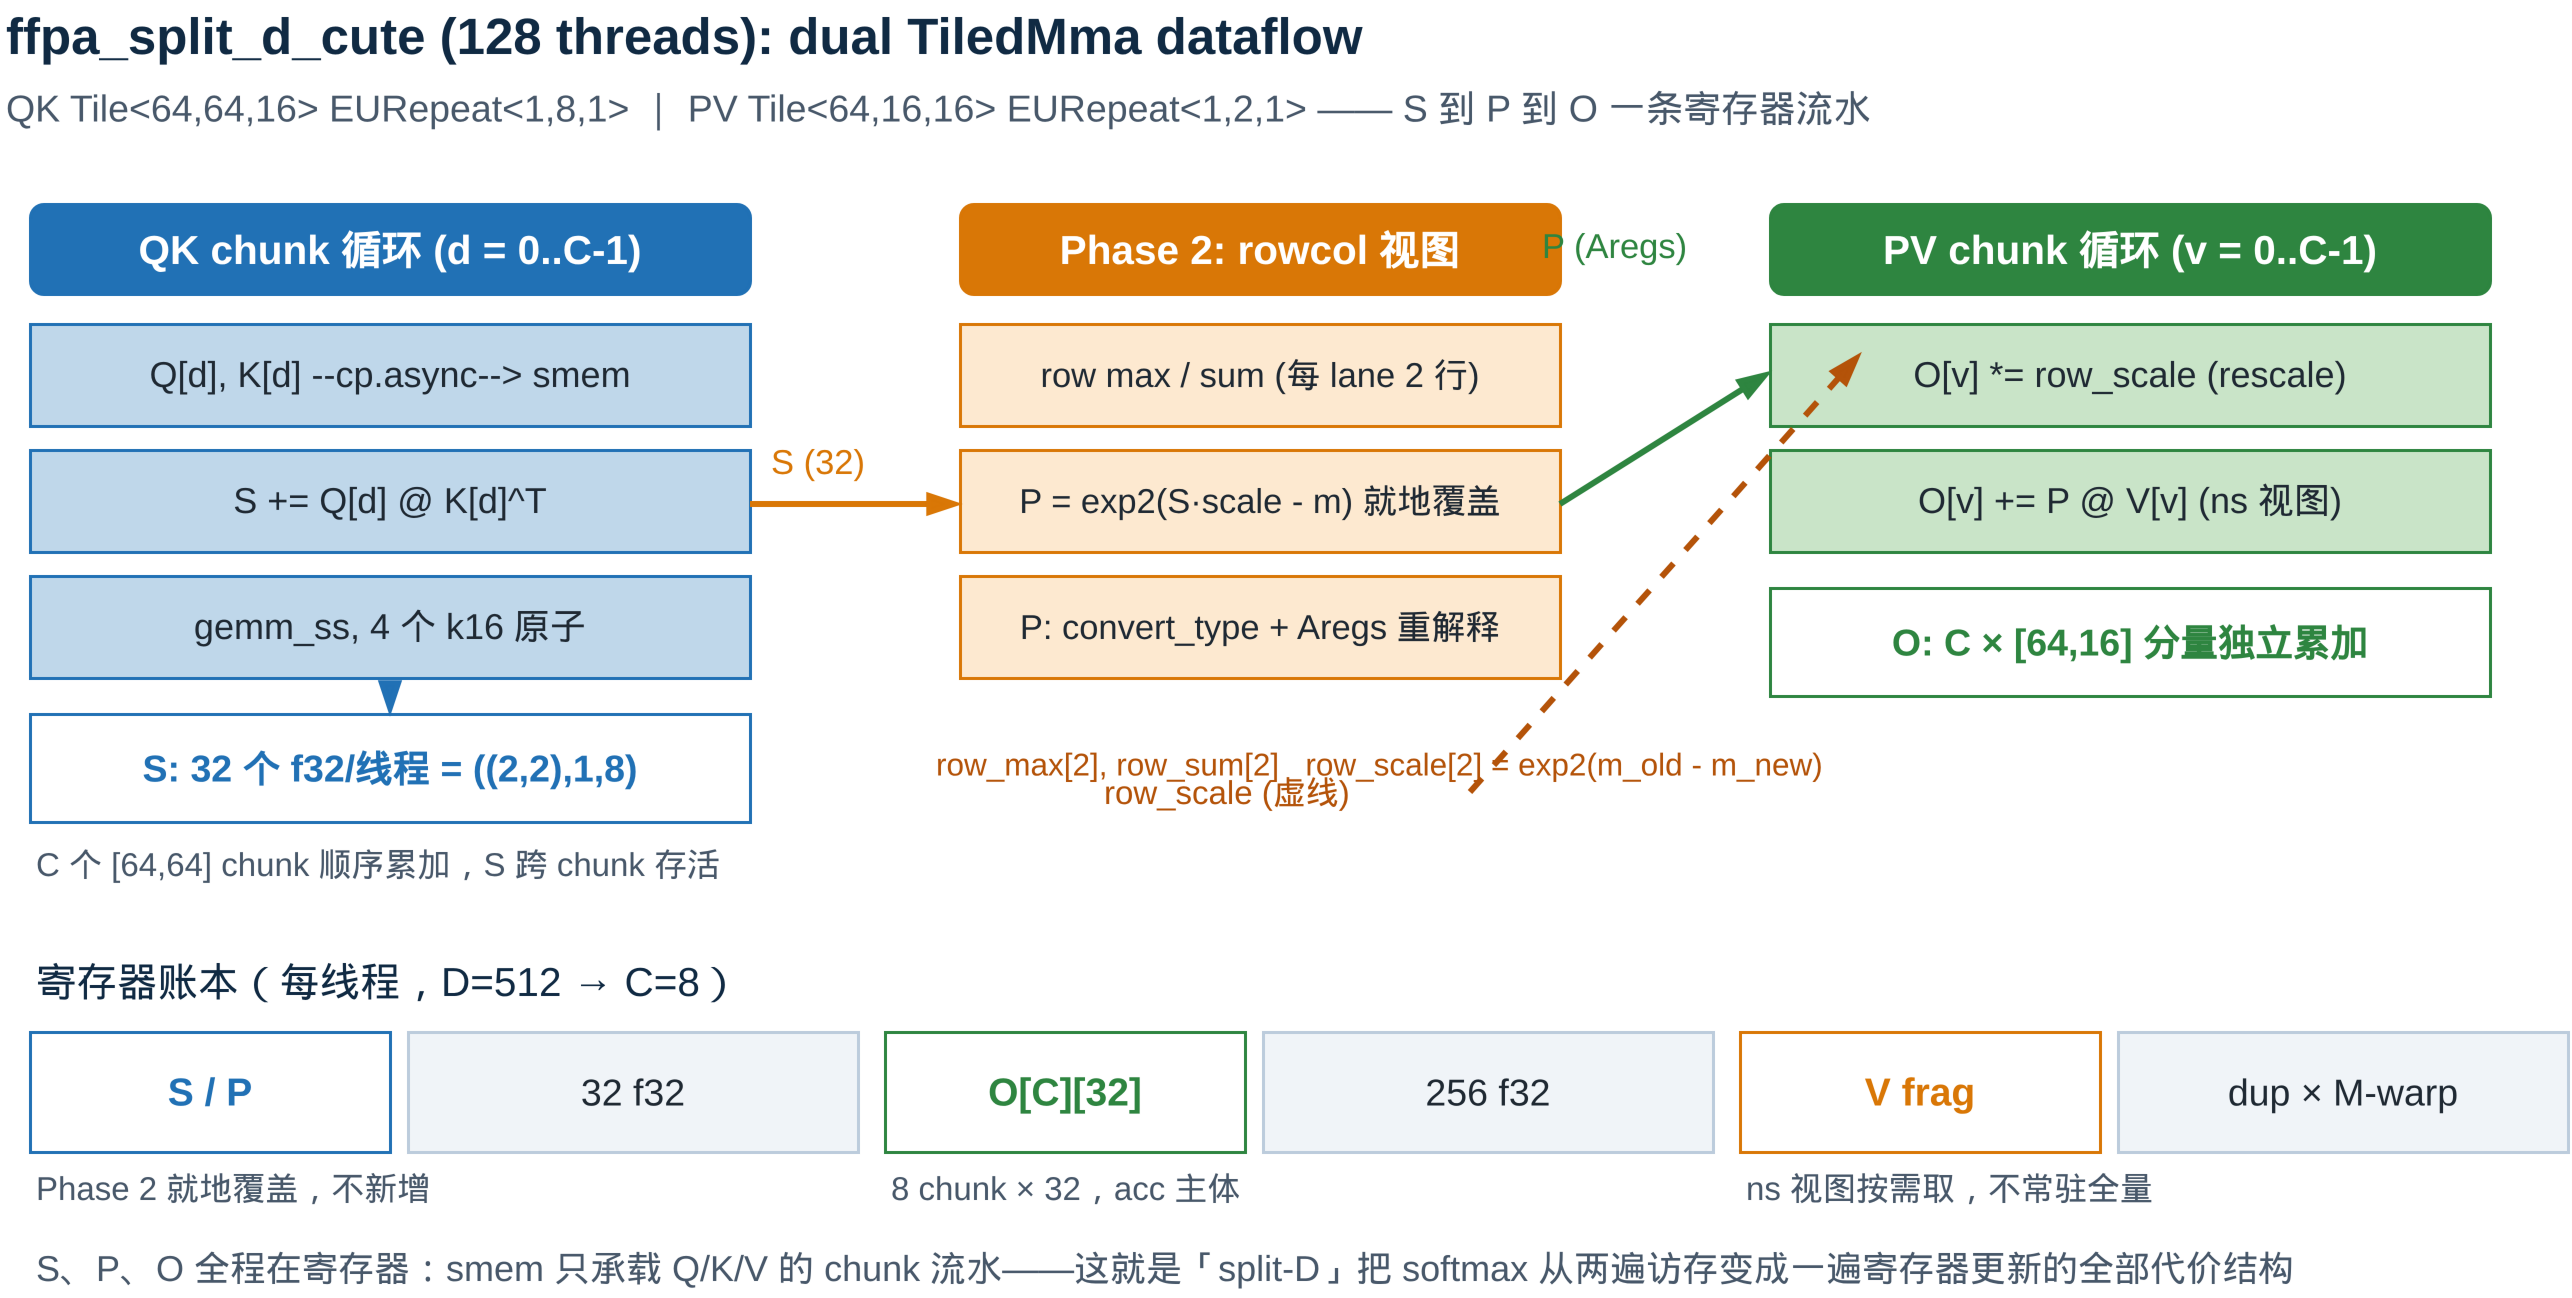
\includegraphics[width=0.92\textwidth]{figures/drawio/fig-26-1-dual-mma/fig-26-1.png}
\begin{tikzpicture}[font=\tiny, >=Stealth,
  hb/.style={align=center, inner sep=2pt, font=\bfseries\fontsize{4.6}{5.2}\selectfont},
  bx/.style={align=center, inner sep=2pt, font=\fontsize{4.2}{4.8}\selectfont},
  tx/.style={align=left, inner sep=1pt, font=\fontsize{4.2}{4.8}\selectfont, anchor=west},
]
  % 左栏：QK chunk 循环（S 累加器跨 chunk 存活）
  \node[hb, fill=tkBlue, text=white, text width=4.20cm] at (2.10,-0.12)
    {QK chunk 循环（$d = 0..C{-}1$）};
  \node[bx, draw=tkBlue, fill=tkFillBlue, text width=3.90cm] at (2.10,-0.75)
    {Q[$d$], K[$d$] $\xrightarrow{\texttt{cp.async}}$ smem};
  \node[bx, draw=tkBlue, fill=tkFillBlue, text width=3.90cm] at (2.10,-1.51)
    {S $+=$ Q[$d$] @ K[$d$]$^{\top}$};
  \node[bx, draw=tkBlue, fill=tkFillBlue, text width=3.90cm] at (2.10,-2.27)
    {gemm\_ss，4 个 k16 原子};
  \node[bx, draw=tkBlue, fill=white, text=tkBlue, text width=3.90cm,
    font=\bfseries\fontsize{4.2}{4.8}\selectfont] at (2.10,-3.03)
    {S：32 个 f32/线程 $=$ ((2,2),1,8)};
  \node[tx, text width=4.20cm] at (0,-3.55)
    {C 个 [64,64] chunk 顺序累加，S 跨 chunk 存活};
  % 中栏：Phase 2（rowcol 视图上的 softmax）
  \node[hb, fill=tkOrange, text=white, text width=3.60cm] at (6.90,-0.12)
    {Phase 2：rowcol 视图};
  \node[bx, draw=tkOrange, fill=tkFillOrange, text width=3.30cm] at (6.90,-0.75)
    {row max / sum（每 lane 2 行）};
  \node[bx, draw=tkOrange, fill=tkFillOrange, text width=3.30cm] at (6.90,-1.51)
    {scores $=$ exp2(S$\cdot$scale $-$ m) 写回 S};
  \node[bx, draw=tkOrange, fill=tkFillOrange, text width=3.30cm] at (6.90,-2.27)
    {P：convert\_type $+$ Aregs 重解释};
  \node[bx, text=tkOrange!80!black, text width=4.30cm] at (6.90,-3.05)
    {row\_max[2], row\_sum[2]\\row\_scale[2] $=$ exp2($m_{\mathrm{old}} - m_{\mathrm{new}}$)};
  % 右栏：PV chunk 循环（O 分量独立 rescale 与累加）
  \node[hb, fill=tkGreen, text=white, text width=4.20cm] at (12.30,-0.12)
    {PV chunk 循环（$v = 0..C{-}1$）};
  \node[bx, draw=tkGreen, fill=tkFillGreen, text width=3.90cm] at (12.30,-0.75)
    {O[$v$] $*=$ row\_scale（rescale）};
  \node[bx, draw=tkGreen, fill=tkFillGreen, text width=3.90cm] at (12.30,-1.51)
    {O[$v$] $+=$ P @ V[$v$]（ns 视图）};
  \node[bx, draw=tkGreen, fill=white, text=tkGreen, text width=3.90cm,
    font=\bfseries\fontsize{4.2}{4.8}\selectfont] at (12.30,-2.27)
    {O：$C \times$ [64,16] 分量独立累加};
  % 主数据流箭头：S -> Phase 2 -> P -> PV
  \draw[->, tkOrange, semithick] (4.28,-1.45) -- (5.02,-1.45);
  \node[tx, text=tkOrange] at (4.35,-1.28) {S (32)};
  \draw[->, tkGreen, semithick] (8.78,-1.45) -- (10.18,-1.45);
  \node[tx, text=tkGreen] at (8.85,-1.28) {P (Aregs)};
  % row_scale 虚线耦合：Phase 2 尾部 -> PV 的 rescale 框
  \draw[->, dashed, tkOrange!80!black, semithick]
    (7.90,-3.42) -- (10.18,-3.42) -- (10.18,-2.42) -- (10.28,-2.42);
  \node[align=center, inner sep=1pt, font=\fontsize{4.2}{4.8}\selectfont,
    text=tkOrange!80!black] at (9.30,-3.68) {row\_scale（虚线）};
  % 底部：寄存器占用
  \node[font=\bfseries\fontsize{4.6}{5.2}\selectfont, anchor=west] at (0,-4.10)
    {寄存器占用（每线程，$D=512 \to C=8$）};
  \node[bx, draw=tkBlue, fill=white, text=tkBlue, text width=1.30cm,
    font=\bfseries\fontsize{4.2}{4.8}\selectfont] at (0.75,-4.55) {S $\to$ P};
  \node[bx, draw=gray!60, fill=gray!12, text width=2.10cm] at (2.90,-4.55) {32 f32 / 32 f16};
  \node[tx, text width=4.2cm] at (0,-4.92) {softmax 写回 S；convert\_type 生成新 P fragment};
  \node[bx, draw=tkGreen, fill=white, text=tkGreen, text width=1.30cm,
    font=\bfseries\fontsize{4.2}{4.8}\selectfont] at (5.95,-4.55) {O[$C$][32]};
  \node[bx, draw=gray!60, fill=gray!12, text width=2.10cm] at (8.10,-4.55) {256 f32 逻辑值（spill）};
  \node[tx] at (5.20,-4.92) {8$\times$32，已超 255 寄存器上限};
  \node[bx, draw=tkOrange, fill=white, text=tkOrange!80!black, text width=1.30cm,
    font=\bfseries\fontsize{4.2}{4.8}\selectfont] at (11.15,-4.55) {V frag};
  \node[bx, draw=gray!60, fill=gray!12, text width=2.10cm] at (13.30,-4.55) {每 M-warp 各一份};
  \node[tx] at (10.40,-4.92) {每线程私有，跨 warp 重复};
  \node[tx, text width=15.0cm] at (0,-5.35)
    {S/P 的更新在寄存器路径，O 的 256 个逻辑值超过 255 上限会 spill；smem 只承载 Q/K/V 的 chunk 流水——
     这就是\textbf{split-D}把 softmax 从两遍访存变成一遍寄存器更新的代价所在};
\end{tikzpicture}
\caption{双 TiledMma 的数据流：QK 沿 $D$ 累加成 $S$（32 个 f32 寄存器跨
chunk 存活），softmax 写回 $S$，再由 \texttt{convert\_type} 产生 f16 $P$，
Aregs 重解释其布局后交给 PV；$O$ 的每个 chunk 分量独立 rescale 与累加，
\texttt{row\_scale}（虚线）耦合两个循环。底部为寄存器占用：$S$ 为 32 个
f32、$P$ 为新生成的 32 个 f16 逻辑值；$O[C][32]$ 共 256 个 f32 逻辑值
（$C{=}8$，已超过 255 个寄存器的硬上限，会 spill）、V fragment 在每个
M-warp 中各有一份私有副本——smem 只承载 Q/K/V 的 chunk 流水。}
\label{fig:26-1}
\end{figure}

\section{性能分析}

本章不给新的实测数字，原因与第~\ref{ch:25}~章相同：本机没有复测 FFPA 的
完整 bench（第~\ref{ch:19}~章给出其性能数据与口径）。这里只做两件事：转录
源码注释里的既有声明（注明出处），并从本章的类型视角讨论 Split-D 抽象层的
运行时成本结构。

源码头注释（\texttt{ffpa\_\allowbreak{}attn.\allowbreak{}cuh} L16--17）的性能声明是：

\begin{quote}
  \textit{性能 (B=1,H=32,N=8192,D=512, SM120a RTX PRO 5000):
  cuDNN SDPA: 57.2 TFLOPS | FFPA TMA WS: 110.7 TFLOPS (1.94x)}
\end{quote}

读数时注意三点口径。（1）这是 TMA + WS 版（256 线程、双角色）的数字，不是
本章精读的 cp.async 版。（2）设备标称 SM120a RTX PRO 5000，而本仓库 README 的
同类标称常写 RTX 5090，同一 sm120 家族的两种卡，绝对值不可直接互比
（第~\ref{ch:19}~章的核对与 CHECKLOG 记录同此）。（3）1.94x 是相对 cuDNN SDPA
的加速比，比较对象与精度配置（f16 输入、f32 累加）需与 bench 脚本核对后才可
引用。

从类型视角看，Split-D 的抽象开销可以逐项归零：

\begin{itemize}[itemsep=2pt,topsep=2pt]
  \item \texttt{kDChunks}、\texttt{k\allowbreak{}QChunk\allowbreak{}Elements} 等全是
        \texttt{constexpr}，chunk 循环的步长、stage 偏移、池大小都在编译期
        折叠成立即数，运行时（在开启优化后）与手写版本无差别。
  \item \texttt{local\_tile}/\texttt{partition\_*} 的坐标算术全部由模板
        推导，编译产物里剩下的是少数 \texttt{mad} 与常量偏移。
  \item 实际的运行时成本在算法侧（chunk 循环的额外 barrier、V 的重复加载），
        与用不用 CuTe 无关。第~\ref{ch:19}~章对这两项开销的量化结论是
        \textbf{Stage 上限压到 2--3，同步开销主导}。
\end{itemize}

CuTe 在 Split-D 上的收益与代价都不在运行时，而在类型可断言：本章测试
（26.9 节）能在不启动 kernel 的情况下核对双 TiledMma 的每条推导。

\section{常见坑}

\textbf{坑一：推 V 的 fragment 布局必须去掉 swizzle。}
\texttt{partition\_\allowbreak{}fragment\_\allowbreak{}B} 要的是值的线程归属，而 swizzle 只改变
元素的 smem 地址。直接用带 SW128 的 \texttt{Smem\allowbreak{}Layout\allowbreak{}Vt} 去推，XOR
置换会混进逻辑坐标，fragment 布局与真值错位：正确做法是
\texttt{get\_\allowbreak{}nonswizzle\_\allowbreak{}portion} 之后再推（L137--141）。但 S2R 的
smem 地址仍由 \texttt{s2r\_thr\_v.partition\_S(sVt\_stg)} 用带 swizzle 的 storage
视图计算，两份视图职责不同。

\textbf{坑二：\texttt{convert\_\allowbreak{}type} 与 \texttt{Aregs} 的区别。}
当前源码先做类型转换、再做布局重解释（L301--303）。但
\texttt{NumericArrayConverter} 只看底层平坦数组，不按 layout 的连续段
分组；Aregs 只换索引。不能用“反序会转换错误分组”解释这段顺序，也不能
把 f32$\to$f16 的转换称为原寄存器零拷贝。

\textbf{坑三：\texttt{o\_\allowbreak{}acc\_\allowbreak{}storage} 的初始化在 chunk 循环外、只做一次。}
它在每个 kv\_tile 迭代里都是\emph{累加}目标，清零只在 kernel 开头
（L174--176）。若把它挪进 kv\_tile 循环，$O$ 会丢失历史。

\textbf{坑四：\texttt{v\_write\_pv} 的初值必须与 Phase 0 的预取数对接。}
Phase 0 写了 $\mathrm{Sv}-1$ 个 chunk，PV 循环从槽位号
$(\mathrm{Sv}-1)\bmod \mathrm{Sv}$ 继续（L308）。改 Phase 0 的预取个数
而忘了这里，会写坏正在被读的 chunk。

\textbf{坑五：chunk 循环里的 \texttt{\_\allowbreak{}\_\allowbreak{}syncthreads\allowbreak{}()} 属于槽位复用协议。}
QK 每轮末尾（L269）与 PV 每轮末尾（L350）的同步不是可有可无的：它们保证本轮
读过的 smem 槽位在下一轮被覆写之前所有线程都已读完；删掉它，表现是
高频偶发数值错误，且随 stage 数增大而加剧。

\textbf{坑六：行状态只有 2 个，但列有 16 个：shfl 掩码只到 2。}
\texttt{row\_max}/\texttt{row\_sum} 的长度是 \texttt{kORows}$=2$，
行内归约靠 \texttt{\_\allowbreak{}\_\allowbreak{}shfl\_\allowbreak{}xor\_\allowbreak{}sync} 的掩码 1 与 2（4 个 lane 一组，
L281--282 与 L291--292）。多加一层掩码 4 会把\emph{另一个 warp 段}的行
卷进来（warp 内 8 个 lane 组对应 8 个不同行块），数值立刻错。

\textbf{坑七：chunk 宽度、smem 池、TMA box 三者必须同步改。}
把 \texttt{kDChunk} 从 64 改成别的值时，SW128 原子、TMA box
（\texttt{Shape\allowbreak{}<\_\allowbreak{}64,\allowbreak{}\_\allowbreak{}64>}）、\texttt{kDChunks} 与 V 的 fragment 预计算
全部要跟着动，一个 64 改三处是这一族 kernel 改动时的固定代价。

\section{面试要点速查}

\begin{enumerate}[itemsep=3pt,topsep=3pt]
  \item \textbf{为什么 QK 的 TiledMma 要 Tile$\langle64,64,16\rangle$，
        而 PV 只要 $\langle64,16,16\rangle$？}
        QK 的 N 向 EURepeat 变成 8，一次覆盖 $S[64,64]$，省掉 N-tile
        循环（提升计算密度）；PV 的累加器 $O$ 要与 chunk 循环的边界对齐，
        小 tile 让 chunk 边界成为寄存器域的边界。两者的 C fragment 大小
        相同（$32$），因为输出形状与线程数相同。
  \item \textbf{Split-D 不改变 fragment 形状是什么意思？}
        $S$ 的 fragment 在 chunk 循环前后都是 $((2,2),1,8)=32$ 个 f32；
        chunk 循环表达的是同一个数组跨迭代累加。变的只是循环结构与
        归约树。
  \item \textbf{$S$ 怎么变成 $P$？为什么不需要 shuffle/smem？}
        先由 \texttt{convert\_type} 做 f32$\to$f16 数值转换并产生新 fragment；
        \texttt{convert\_\allowbreak{}layout\_\allowbreak{}acc\_\allowbreak{}Aregs} 再按 $m16n8$ 的 C 与
        $m16k16$ 的 A 映射重解释布局（C 的列向 2 值 $=$ A 的 K 向 2 值）。
        免掉的是 smem 往返，Aregs 本身仍是不搬数据的布局重解释。SM80
        $k8$ atom 的 A/C 布局相同，可拆两次 PV 继续复用；其他约定要重推。
  \item \textbf{为什么 V 的 fragment 布局要预先算、且用 nonswizzle 版本？}
        循环里只换指针不改布局——算一次省每轮推导；去掉 swizzle 是因为
        它只改地址不改值的线程归属。S2R 的 smem 地址另由
        \texttt{partition\_S} 在带 swizzle 的视图上计算。
  \item \textbf{每个线程持有多少 $O$ 逻辑累加值？}
        $C\times32$ 个 f32 \emph{逻辑累加值}：$D=512$ 时 256 个，已超过
        每线程 255 个寄存器的硬上限，实际需要 spill。第一维来自 chunk
        循环（问题尺寸），第二维来自 fragment 布局（TiledMma）。
  \item \textbf{行归约为什么要用到 \texttt{shfl\_xor} 掩码 1 和 2？}
        $m16n8$ 的 C fragment 里一行由 4 个 lane 拼成（每 lane 2 行 $\times$
        16 列），掩码 1 与 2 恰好把 4 个 lane 的两两组合并；再多就跨行块了。
  \item \textbf{smem 池的偏移为什么用指针算术而不是 layout 的 stage 维？}
        当前实现选择指针算术，不是 CuTe 的必然要求。真实的 stage mode
        应使用 stride 等于一块 chunk 元素数的非零 stride；只有 stride-0
        伪维才表示所有 stage 落到同一元素，从而使 \texttt{cosize} 与
        partition 不再对应池大小。
  \item \textbf{chunk 数与 stage 数是什么关系？}
        正交：chunk 数是问题尺寸（head\_dim/64），stage 数是流水深度
        （smem 预算）。两者的相位关系与约束见第~\ref{ch:19}~章。
\end{enumerate}

\section{最小测试与动手实验}

本章测试（\texttt{tests/\allowbreak{}ch26\_\allowbreak{}ffpa\_\allowbreak{}cute.\allowbreak{}cu}）与前几章的不同之处是
以 host 端类型断言为主：不启动 kernel，只对 traits 与 fragment
做静态/运行时断言，全部来自 26.3 节的代数。下文的实测都指该测试或等价 probe
的 host 端输出：

\begin{enumerate}[itemsep=2pt,topsep=2pt]
  \item \textbf{D-chunk 常量}：对 $D\in\{64,128,192,512\}$ 断言
        \texttt{kDChunks}$=D/64$ 与两个 chunk 池
        $\mathrm{cosize}=64\times64$；
  \item \textbf{双 TiledMma 推导链}：QK 的 \texttt{tile\_\allowbreak{}size\_\allowbreak{}mnk}
        $=(64,64,16)$、PV $=(64,16,16)$，线程数均为 128；
  \item \textbf{fragment 恒等式}：两个
        \texttt{partition\_\allowbreak{}fragment\_\allowbreak{}C}$((64,64))$ 的每线程元素数都是 32。
        rowcol 后的行列数 $(2,16)$；Aregs 重解释前后元素数守恒；
  \item \textbf{switch 语义}：\texttt{local\_tile} 在 $(64,64)$ tile 与
        $(row\_tile, d\_chunk)$ 坐标下的首元素地址等于
        \texttt{row\_\allowbreak{}tile*64*D + d\_\allowbreak{}chunk*64}。
\end{enumerate}

再加两个小规模 kernel 正确性 case（与第~\ref{ch:19}~章的覆盖互不重复）：

\begin{itemize}[itemsep=2pt,topsep=2pt]
  \item case E：$D=192$（3 个 chunk，且与 $\mathrm{Sk}{=}3$ 相等，用来测
        chunk 数 $=$ stage 数的边界；实际预取深度为 $\mathrm{Sk}-1=2$）、$N=128$、$H=2$、
        $\mathrm{Sk}{=}3,\mathrm{Sv}{=}2$；
  \item case F：$D=128$（2 个 chunk，$\mathrm{Sk}{=}2$）、$N=128$、$H=2$。
\end{itemize}

两者都与 CPU fp64 参考对照（容差 \texttt{TOL\_F16ACC}），运行：

\begin{lstlisting}[style=console]
cd book/tests && CUDA_VISIBLE_DEVICES=6 ./build_tests.sh --arch sm_120a --ch ch26
\end{lstlisting}

本机实测输出（sm\_120a，6 号卡）：

{\scriptsize
\begin{lstlisting}[style=console]
PASS case A chunk constants D=64 (kDChunks=1): mismatches=0 (4 checks)
PASS case A chunk constants D=128 (kDChunks=2): mismatches=0 (6 checks)
PASS case A chunk constants D=192 (kDChunks=3): mismatches=0 (8 checks)
PASS case A chunk constants D=512 (kDChunks=8): mismatches=0 (18 checks)
PASS case B dual TiledMma derivation chain (D=512): mismatches=0 (6 checks)
probe: rowcol=(2,16) aregs_elems=32
PASS case B2 device probe: rowcol (2,16) & Aregs 32 elems: mismatches=0 (3 checks)
PASS ffpa split-d cute D=192 N=128 Sk=3 Sv=2 B=1 H=2: max_abs_err=8.481e-05 (tol=5.0e-02)
PASS ffpa split-d cute D=128 N=128 Sk=2 Sv=2 B=1 H=2: max_abs_err=8.084e-05 (tol=5.0e-02)
ALL OK
\end{lstlisting}
}

\section*{延伸阅读}

\begin{itemize}[itemsep=2pt,topsep=2pt]
  \item @竹熙佳处《写给大家看的 CuTe 教程：Layout Compose \& Inverse》——
        $S\to P$ 布局变换的完整讲法（Tri Dao 的几何法与 @reed 的代数法），
        本章 26.3.3 节与第~\ref{ch:25}~章 25.3.4 节的主参考。\\
        \url{https://zhuanlan.zhihu.com/p/1962625273636845008}
  \item @reed《cute 之 高效 GEMM 实现》——TiledMMA 的组装层次、
        多级流水的写法与 Epilogue 的 smem 中转；同系列《cute 之 简单
        GEMM 实现》给出最小版本的组装范式，配合 26.3.1 的推导链与
        26.4 的相位阅读一起看。\\
        \url{https://zhuanlan.zhihu.com/p/675308830}
  \item @竹熙佳处《写给大家看的 CuTe 教程：tiled mma》——fragment 视角的
        线程-值映射，26.3.2 节两个恒等式的入门读物。\\
        \url{https://zhuanlan.zhihu.com/p/1937145378446226159}
  \item @DefTruth《FFPA(Split-D)：FA2 无限 HeadDim 扩展》——
        本主题在中文社区最系统的公开文章，Split-D 的动机与 RD 波形分析
        可与第~\ref{ch:19}~章的推导对读。\\
        \url{https://zhuanlan.zhihu.com/p/13975660308}
  \item @DefTruth《图解：从 Online-Softmax 到 FlashAttention V1/V2/V3》——
        online softmax 的图解（本书第~\ref{ch:15}~章的主参考），
        配合本章 26.3.2 的 rowcol 代数读更佳。\\
        \url{https://zhuanlan.zhihu.com/p/668888063}
  \item @66RING《使用 cutlass cute 复现 flash attention》——CuTe 版 FA 的
        工程化复现，可与第~\ref{ch:25}~章的四个实现对照。\\
        \url{https://zhuanlan.zhihu.com/p/696323042}
  \item @DeclK《CUTLASS CUTE 系列（1--5）》——布局代数与 MMA/COPY 抽象的
        系统性替代读物，作为第~\ref{ch:20}--\ref{ch:22}~章的复习材料。\\
        \url{https://zhuanlan.zhihu.com/p/1983922984805742098}
\end{itemize}
